Para este trabajo se planteó la siguiente pregunta: 

\begin{center}
\textit{``¿Es posible que un satélite orbite en cualquier dirección?''}
\end{center}

Partiendo del lanzamiento del mismo, estos usualmente se lanzan en el sentido en el que la tierra gira, esto para aprovechar la trayectoria que tiene ya que se requiere mucha energía para llegar a la velocidad de la órbita. \\
Esto para ahorrar combustible, haciendo que la velocidad inicial sea útil. Cualquier otra ruta, \textbf{es posible} pero habría que justificar su gasto.\\

Primeramente habría que ver las órbitas que pueden tomar los satélites geoestacionarios (que por definición podrían estar solo sobre el Ecuador ya que es el único eje en el que podrían estar en un mismo punto sobre la tierra en una órbita de $\approx$24hrs). Por otro lado tenemos los geosíncronos, estos al igual que el anterior tienen una órbita de $\approx$24hrs. con la diferencia que puede tener cierto grado de inclinación respecto al ecuador. \\{ }\\
Hasta este punto todo normal, ya que son órbitas que estan en relación al centro de masa de cada uno, de acuerdo a la \textit{Ley Universal de Gravitación de Newton} ($F=G\cdot\frac{m_1\cdot m_2}{r^2}$). \\{ }\\

\textbf{Pero}, \textit{``¿Que pasaría si tuvieramos una órbita del siguiente tipo?''}

\begin{figure}[ht!]
\centering
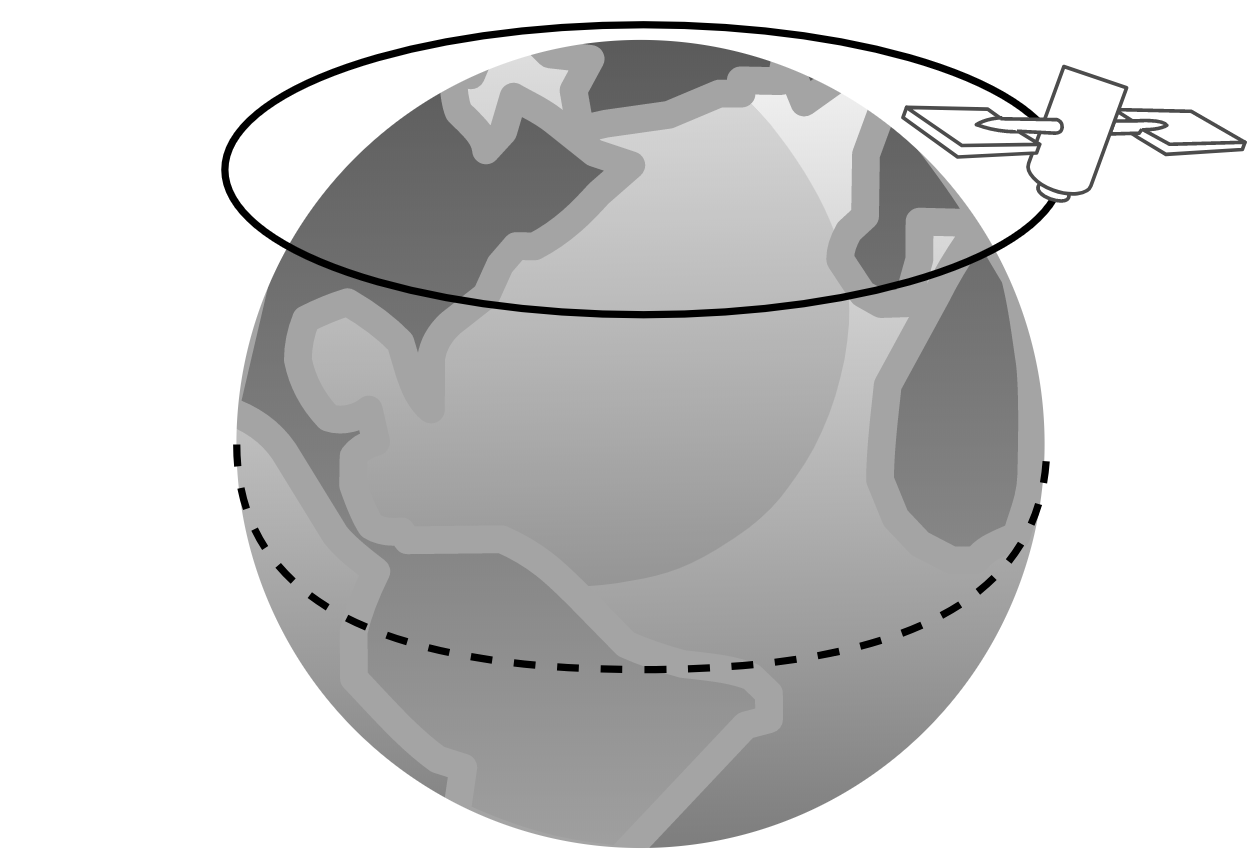
\includegraphics[scale=0.075]{imagenes/paralelo.png}
\end{figure}

Este recorrido es imposible, porque la tierra no está en el \textit{foco de órbita} del satélite. Un movimiento como este no obedecería la ley de Kepler\footnote{Si se lo extendiera, habría que decir que el satélite debería seguir una órbita respecto a uno de sus focos.}. Lo que pasaría es que el satélite se inclinaría. Esta situación no es conveniente para ninguna institución ya que habria que corregir su trayectoria con mayor regularidad. \\{ }\\
Otro tipo de trayectoria que se puede plantear es: 
\begin{center}
 \textit{``Un satélite geoestacionario directamente sobre los polos.''}
\end{center}

\begin{figure}[ht!]
\centering
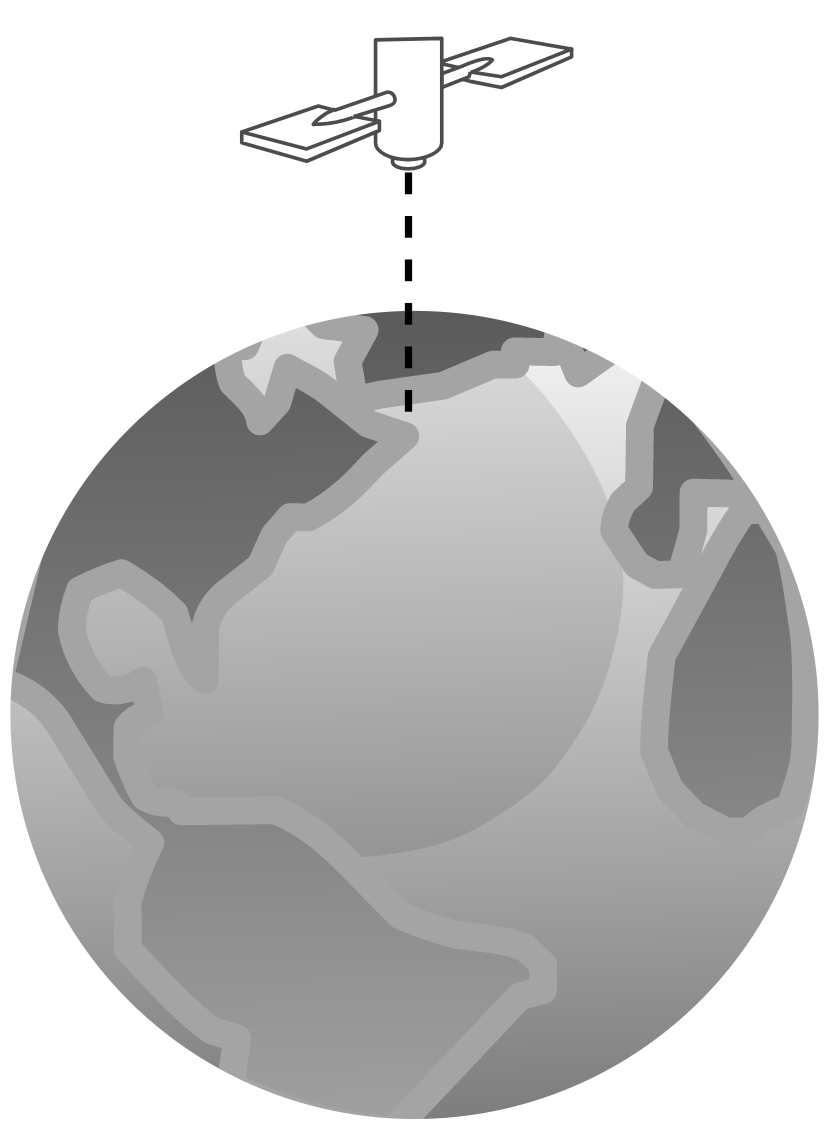
\includegraphics[scale=0.075]{imagenes/polo.png}
\end{figure}

Esto no sería posible ya que el satélite tendría que estar en reposo, esto provocaría que no haya fuerza que lo repela, por lo tanto simplemente cedería a la gravedad. Dicho esto, es posible colocar satélites geosíncronos con órbitas semi polares (es decir con grados de inclinación $0^\circ \leq \theta < 90^\circ$ respecto al Ecuador).